\graphicspath{{figures/coord/}}

%\setcounter{secnumdepth}{0}
\renewcommand{\theequation}{\thechapter.\arabic{equation}}
\renewcommand{\thetheorem}{\thechapter.\arabic{theorem}}
\renewcommand{\thebc}{\thechapter.\arabic{theorem}}
\renewcommand{\theeg}{\thechapter.\arabic{theorem}}
%\counterwithin{theorem}{chapter}
%\numberwithin{theorem}{chapter}


\chapter{3d Coordinate Systems}\label{ap:3dcoord}

\section{Cartesian Coordinates}\label{ap:cartCoord}
Here is a figure showing the definitions of the 
three Cartesian coordinates $(x,y,z)$
\begin{efig}
\begin{center}
    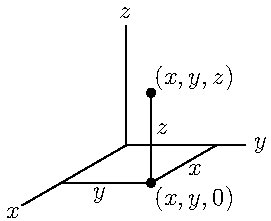
\includegraphics{cart1.pdf}
\end{center}
\end{efig}
and here are three figures showing a surface of constant $x$,
a surface of constant $x$, and a surface of constant $z$.
\begin{wfig}
\begin{center}
    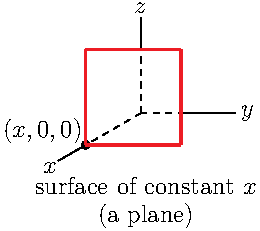
\includegraphics{cart3.pdf}\qquad
    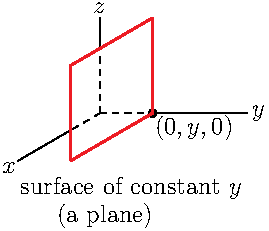
\includegraphics{cart4.pdf}\qquad
    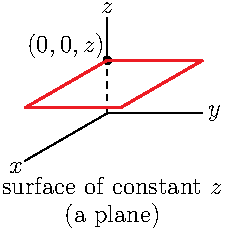
\includegraphics{cart2.pdf}
\end{center}
\end{wfig}
Finally here is a figure showing the volume element $\dee{V}$ in
cartesian coordinates.
\begin{efig}
\begin{center}
    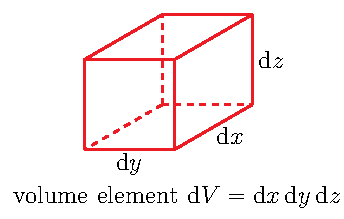
\includegraphics{cart5.pdf}
\end{center}
\end{efig}



\section{Cylindrical Coordinates}\label{ap:cylCoord}

Here is a figure showing the definitions of the 
three cylindrical coordinates 
\begin{align*}
r&=\text{ distance from }(0,0,0)\text{ to }(x,y,0)\\
\theta&=\text{ angle between the the $x$ axis and the line joining $(x,y,0)$ to $(0,0,0)$}\\
z&=\text{ signed distance from }(x,y,z)
\text{ to the $xy$-plane}
\end{align*}
\begin{efig}
\begin{center}
    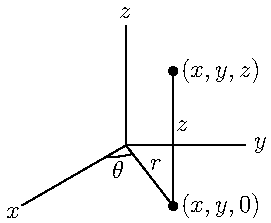
\includegraphics{cyl1.pdf}
\end{center}
\end{efig}
The cartesian and cylindrical coordinates
are related by
\begin{align*}
x&=r\cos\theta &
y&=r\sin\theta &
z&=z \\
    r&=\sqrt{x^2+y^2} &
    \theta&=\arctan\frac{y}{x} &
    z&=z
\end{align*}
Here are three figures showing a surface of constant $r$,
a surface of constant $\theta$, and a surface of constant $z$.
\begin{wfig}
\begin{center}
    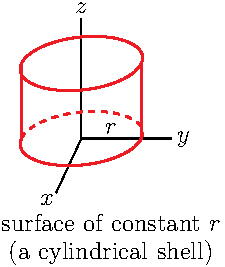
\includegraphics{cyl3.pdf}\qquad
    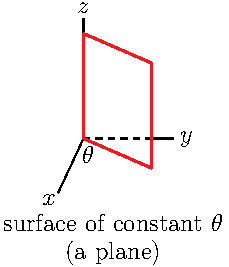
\includegraphics{cyl4.pdf}\qquad
    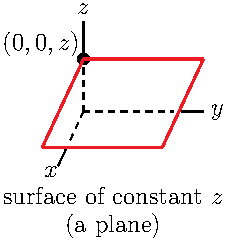
\includegraphics{cyl2.pdf}
\end{center}
\end{wfig}
Finally here is a figure showing the volume element $\dee{V}$ in
cylindrical coordinates.
\begin{efig}
\begin{center}
    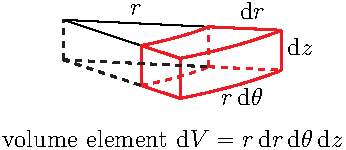
\includegraphics{cyl5.pdf}
\end{center}
\end{efig}





\section{Spherical Coordinates}\label{ap:spherCoord}

Here is a figure showing the definitions of the 
three spherical coordinates 
\begin{align*}
\rho&=\text{ distance from }(0,0,0)\text{ to }(x,y,z)\\
\varphi&=\text{ angle between the $z$ axis and the line joining $(x,y,z)$ to $(0,0,0)$} \\
\theta&=\text{ angle between the $x$ axis and the line joining $(x,y,0)$ to $(0,0,0)$}
%\varphi&=\text{ angle between the line }\overline{(0,0,0)\,(x,y,z)}
%\text{ and the $z$ axis}\\
%\theta&=\text{ angle between the line }\overline{(0,0,0)\,(x,y,0)}
%\text{ and the $x$ axis}
\end{align*}
\begin{efig}
\begin{center}
    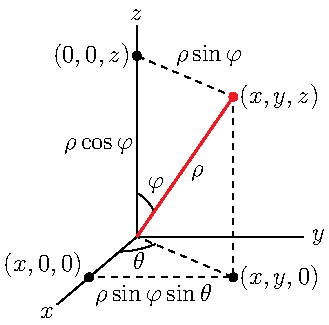
\includegraphics{spherical.pdf}
\end{center}
\end{efig}
and here are two more figures giving the side and top views of the 
previous figure.
\begin{efig}
\begin{center}
    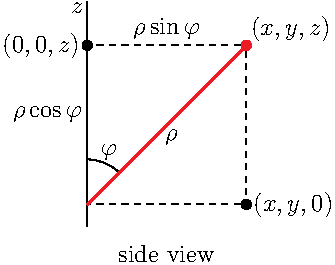
\includegraphics{sphericalSide.pdf}\qquad
    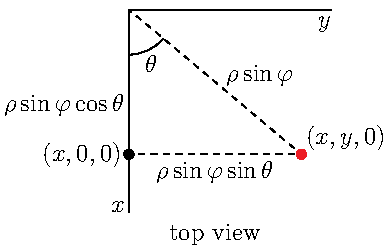
\includegraphics{sphericalTop.pdf}\qquad
\end{center}
\end{efig}
The cartesian and spherical coordinates
are related by
\begin{align*}
x&=\rho\sin\varphi\cos\theta &
y&=\rho\sin\varphi\sin\theta &
z&=\rho\cos\varphi \\
 \rho&=\sqrt{x^2+y^2+z^2} &
 \theta&=\arctan\frac{y}{x} &
 \varphi&=\arctan\frac{\sqrt{x^2+y^2}}{z}
\end{align*}
Here are three figures showing a surface of constant $\rho$,
a surface of constant $\theta$, and a surface of constant $\varphi$.
\begin{wfig}
\begin{center}
    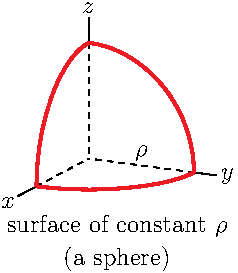
\includegraphics{spher2.pdf}\qquad
    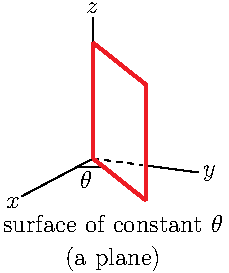
\includegraphics{spher3.pdf}\qquad
    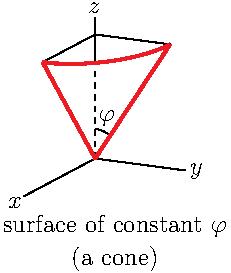
\includegraphics{spher4.pdf}
\end{center}
\end{wfig}
Here is a figure showing the surface element $\dee{S}$ in
spherical coordinates
\begin{efig}
\begin{center}
    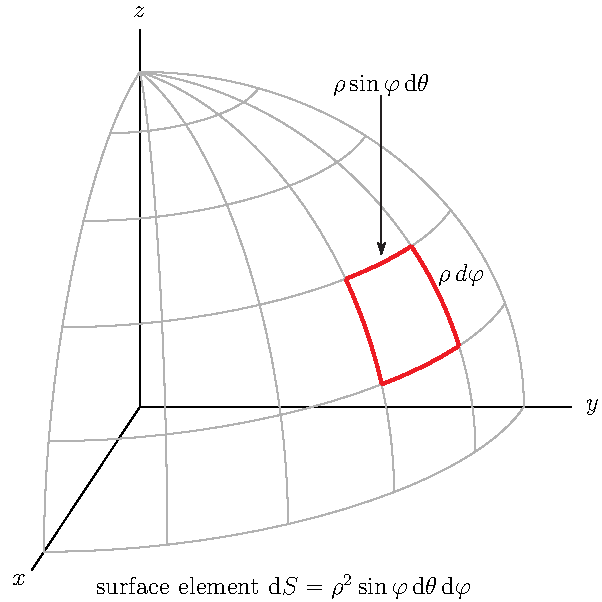
\includegraphics{spher11.pdf}
\end{center}
\end{efig}
and two extracts of the above figure to make it easier to see 
how the factors $\rho\ \dee{\varphi}$ and 
$\rho\sin\varphi\ \dee{\theta}$ arise.
\begin{wfig}
\begin{center}
    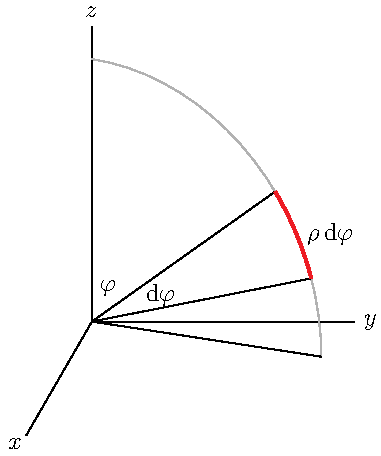
\includegraphics{spher9.pdf}\qquad
    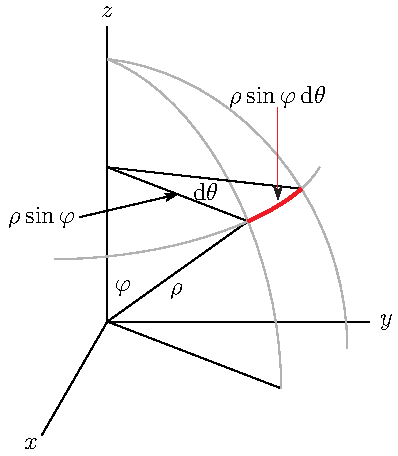
\includegraphics{spher10.pdf}
\end{center}
\end{wfig}
Finally, here is a figure showing the volume element $\dee{V}$ in
spherical coordinates
\begin{efig}
\begin{center}
    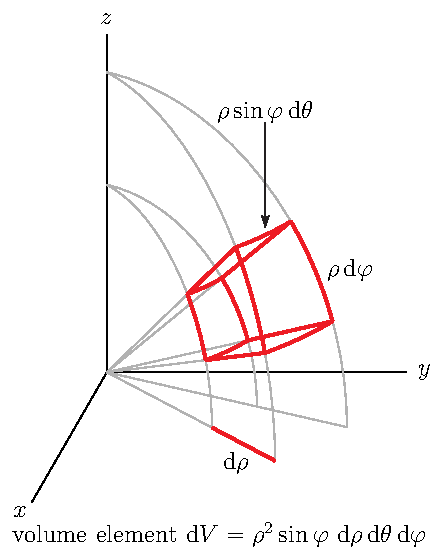
\includegraphics{spher5.pdf}
\end{center}
\end{efig}
%and two extracts of the above figure to make it easier to see 
%how $\rho\ \dee{\varphi}$ and $\rho\sin\varphi\ \dee{\theta}$ arise.
%\begin{wfig}
%\begin{center}
%    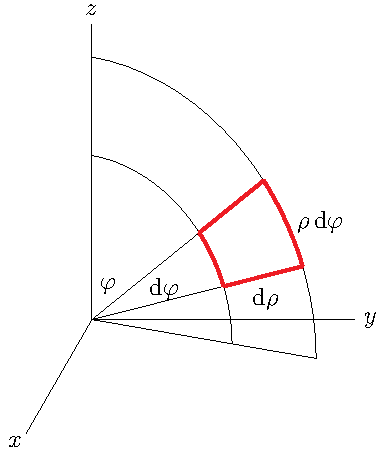
\includegraphics{spher6.pdf}\qquad
%    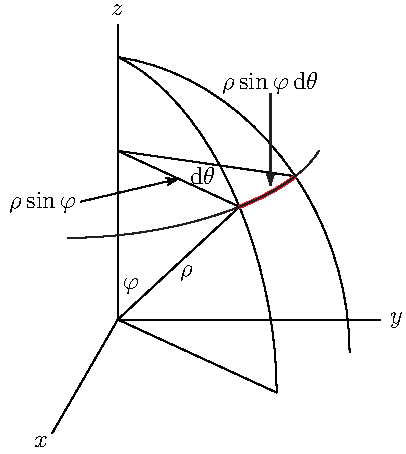
\includegraphics{spher7.pdf}
%\end{center}
%\end{wfig}




